\documentclass{article}
\usepackage{graphicx}

\begin{document}

The basic idea was to caculate the the integral of the function
$$y = x^3 + x^{2/3}$$
This was done both numerically as well as analytically.

For the numerical integration, Simpson's rule was used:
$$\int_a^b f(x) dx \approx {(b-a)\over 6} \left(y(a) + 4 y((a+b)/2) + y(b)\right)$$

For the analytical integration, the result is given by:

$$\int_a^b f(x) dx = x^4/4 + 3/5 x^{5/3} |_a^b$$

The integral was computed between 0 and 10. The numerical integration was
about 0.02\% off from the analytical one.

I then proceded to split the Simpson's integration up into multiple steps, 
and calculated the fractional error as a function of the number of pieces.
The results are shown in Figure \ref{fig:simp}

\begin{figure}
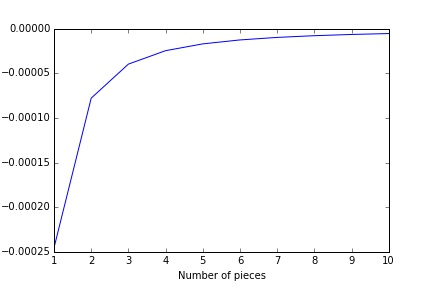
\includegraphics[width=\textwidth]{../q3/simp.jpg}
\caption{Fractional error of numerical integration as a function of
number of intervals.}
\label{fig:simp}
\end{figure}

Table \ref{tab:simp} shows the fractional error as a function of the number
of pieces:

\begin{table}
\begin{tabular}{ll}
Number of pieces & Fractional error \\
1 & -0.000245307331841 \\
2 & -7.7656140706e-05 \\
3 & -3.95427362471e-05 \\
4 & -2.44881707436e-05 \\
5 & -1.68846338361e-05 \\
6 & -1.24609013845e-05 \\
7 & -9.63799435511e-06 \\
8 & -7.71512276632e-06 \\
9 & -6.34008146724e-06 \\
10 & -5.31908134828e-06 \\
\end{tabular}
\caption{Fractional error as a function of number of pieces}
\label{tab:simp}
\end{table}

\end{document}
